\documentclass[12pt]{report}

% Required Packages
\usepackage[utf8]{inputenc}
\usepackage[titletoc]{appendix}
\usepackage{multirow}
\usepackage{caption}
\usepackage{tikz}
\usepackage{tabularx}
\usepackage{url}
\usepackage{ifthen}
\usepackage{verbatim}
\usepackage{blindtext}
\usepackage{amsmath}
\usepackage{natbib}
\usepackage{textcomp}
\usepackage{footnote}
\usepackage[hypertexnames=false,linktocpage=true]{hyperref}
\hypersetup{colorlinks=true,linkcolor=blue,anchorcolor=blue,citecolor=blue,filecolor=blue,urlcolor=blue,bookmarksnumbered=true,pdfview=FitB}

\graphicspath{ {images/} }

% Set ISU required margins for unbound manuscript.
\usepackage[margin=1.0in]{geometry}

% Allow frontmatter and mainmatter in an article instead of a book.
\newcommand\frontmatter{%
    \cleardoublepage
    \pagenumbering{roman}}
\newcommand\mainmatter{%
    \cleardoublepage
    \pagenumbering{arabic}}

% ISU thesis wants specific ToC formatting.
\usepackage{tocloft}
\renewcommand{\contentsname}{\hfill\bfseries\Large TABLE OF CONTENTS\hfill}
\renewcommand\cftaftertoctitle{\hfill}
\renewcommand\cftchapfont{\bfseries\MakeUppercase}
\renewcommand\cftchappresnum{\chaptername~}
\renewcommand\cftchapaftersnum{.}
\cftsetindents{chapter}{0em}{8em}
\cftsetindents{section}{2em}{6em}
\cftsetindents{subsection}{4em}{6em}

% ISU thesis wants bold, centered, uppercase chapters.
\usepackage{titlesec}
\titleformat{\chapter}[display]
    {\normalfont\Large\bfseries\centering}
    {\MakeUppercase\chaptertitlename\ \thechapter}{0pt}{\Large\uppercase}
\titlespacing*{\chapter}{0pt}{-30pt}{30pt}

% ISU thesis wants bold, centered, IntialCaps sections.
\titleformat{\section}[display]
    {\normalfont\large\bfseries\centering}
    {}{0pt}{\large}

% ISU wants 16pt Chapters and 12pt text.
% That makes for 14pt sections.
\makeatletter
\renewcommand\Large{\@setfontsize\Large\@xivpt{16}}
\renewcommand\large{\@setfontsize\Large\@xivpt{14}}
\makeatother

% ISU wants double spacing.
\usepackage{setspace}

% ISU examples show indents in paragraphs even after centered headings.
\usepackage{indentfirst}

% ISU wants page numbers top and centered.
\usepackage{fancyhdr}
\pagestyle{fancy}
\fancyhf{} % Clear all headers and footers.
\fancyhead[C]{\textbf{\thepage}} % Put page # at top of page.
\fancypagestyle{plain}{ % Do the same thing for the plain style.
    \fancyhf{} 
    \fancyhead[C]{\textbf{\thepage}}
    }
\renewcommand{\headrulewidth}{0pt}

% Include tables and figures.
\newcommand{\showtablesandfigures}{}

% A bit of hacking to get custom g3 article environments
% to typeset without including g3 styles.
\newcommand{\header}{}
\newenvironment*{tableminipage}[1]{}{}

% Make LaTeX look nice in the paper.
\usepackage{xspace}
\newcommand{\latex}{\LaTeX\xspace}


\begin{document}
\frontmatter
\title{Genomic Prediction with Neural Networks}
\author{Riley McDowell}
\date{\today}
\maketitle

\setcounter{page}{2}
\tableofcontents{}


\doublespacing
\phantomsection
\chapter*{Abstract}

Reduced costs for DNA marker technology coupled has generated a huge amount of
molecular data and greatly increased the options available to characterize lines 
in a breeding program. Concurrently, the field of machine learning under
the moniker of data science has experienced a resurgence of research into 
techniques to detect or "learn" patterns in noisy data in a variety of 
technical applications. Here, we present a review of current genomic prediction 
and machine learning literature. We apply so called "deep learning"
techniques from machine learning research related to regularized neural networks to six 
phenotypic prediction tasks from published reference datasets. 
The neural network models are compared to a selection of regularized bayesian 
and linear regression techniques commonly employed for phenotypic prediction and genomic
selection tasks. Applying regularization frequently improves neural network 
prediction accuracy. On three prediction tasks, regularized neural networks 
are the most accurate model evaluated. The depth of the network archetecture
does not appear to influence the accuracy of the trained model. We also find
that concerns about the computer processing time needed to train neural network 
models to perform well in genomic prediction tasks may not apply when Graphics
Processing Units are used for model training.


%The abstract should be written for people who may not read the 
%entire paper, so it must stand on its own.  The impression it makes usually determines 
%whether the reader will go on to read the article, so the abstract must be 
%engaging, clear, and concise.  In addition, the abstract may be the only part of the 
%article that is indexed in databases, so it must accurately reflect the 
%content of the article. A well-written abstract is the  most effective way to reach intended 
%readers, leading to more robust search, retrieval, and usage of the article. 


\addcontentsline{toc}{chapter}{Abstract}


\mainmatter
% Chapter #1 - General Introduction
\chapter{General Introduction} \label{chp:gen-intro}

\section{Introduction} \label{sec:gen-intro}

Humans have been breeding plants for food since the dawn of agriculture. This process
emerged from a haphazard form of artificial selection where farmers would save seed from the 
highest yielding, healthiest, and easiest to harvest plants to harvest the following year. 
Over thousands of years, this process produced many of the subspecies of plants of  
agricultural value today.

% Wikipedia Green revolution article.
Between 1930 and 1960, academic agricultural and plant breeding communities were setting the
stage for agricultural giants such as Norman Borlaug, Henry A. Wallace, and others explored 
options to breed plants for specific traits, and apply rigorous, scientifically-motivated 
management practices which improve varieties and the yield of agriculture practice worldwide.

As an example, in 1930, corn was an open-pollinated crop with an average 
yield around 20-30 bu/ac. By 1960, field corn had was usually single-cross hybrids 
producing twice the yield of those bred only two or three decades earlier. The implementation
agricultural practices that would drive the green revolution had been kicked off, and
the stage was set for a rapid improvement in yield and genetic gain year-over-year in
corn as well as many other crops. This improvement continued into the 2000s \citep{evenson2003}.

The green revolution drove crop production yields higher through a combination of 
improved agricultural practices and varieties that had greater yield potential
and agronomic stability. By the year 2000, advances in agronomy were slowing, and 
molecular breeding technologies were promising the next advancement in crop yield
through a focus on a better understanding of crop DNA. The advent of Bt Corn was the
landmark technology delivering on the promise of biotechnology in agriculture.
Bt corn was first commercialized in in 1996 and accounted for 63\% of U.S. grain 
corn by 2010 \citep{fernandez2012}. 

Biotechnology in agriculture is not limited only to transgenic traits. The cost of 
DNA sequencing and genetic marker assays began to fall during as the green revolution
came to a close. The cost of SNP assays has dropped so sharply that today it is 
possible to apply them to many thousands of samples in large breeding programs \citep{hiremath2012}. 
In many cases, it is less costly to genotype a seed than to grow it and observe its phenotype.

Because a SNP assay captures the genes and thus a part of the genetic potential of an 
individual, it is be possible to use the outcome of a SNP assay to predict the genetic
potential of the sampled individual in a affordable way. This process is known 
as genomic prediction, and when used to inform breeding 
program selections is known as genomic selection. Genomic prediction is typically 
applied early in a breeding program as a way to increase the overall selection 
pressure in a breeding program to increase genetic gain. A review of literature
and methods to perform this technique is presented in Section \ref{sec:lit-review}. 

The genetic gain in a breeding program is directly related to a host of factors. A 
general guideline to expected genetic gain each year in an inbred breeding 
program is presented in Equation \ref{eq:genetic_gain} \citep{fehr1987}. The equation is
often used as a general guideline to explore whether changes in breeding strategy will
have a positive or negative effect on genetic gain. 

\begin{equation} \label{eq:genetic_gain}
\begin{split}
    G_y           &= \textrm{genetic gain per year} \\
    k             &= \textrm{selection differential} \\
    r             &= \textrm{number of replications} \\
    t             &= \textrm{number of environments} \\
    n             &= \textrm{plants per plot} \\
    \sigma^2_{A}  &= \textrm{additive genetic variation} \\
    \sigma^2_{u}  &= \textrm{within-plot environmental variation} \\
    \sigma^2_{wg} &= \textrm{within-plot genetic variation} \\
    \sigma^2      &= \textrm{between-plot variation} \\
    \sigma^2_{ge} &= \textrm{genotype by environment interaction variation} \\
    \sigma^2_{g}  &= \textrm{genotypic variation} \\
    G_y           &= \frac{k\sigma^2_A}{y \sqrt{ \frac{\frac{\sigma^2_{u} + \sigma^2_{wg}}{n} + \sigma^2}{rt} + \frac{\sigma^2_{ge}}{t} + \sigma^2_{g} }} \\
\end{split}
\end{equation}

From Equation \ref{eq:genetic_gain}, it is clear that improvements in genetic gain per year can
be made by increasing the number of replications and/or environments tested, increasing the 
number of plants within each experimental plot, or increasing overall selection pressure 
during the breeding program. Genomic selection improves genetic gain by addressing 
all of these at once.

\begin{itemize}
    \item A breeder may grow many more plants than can be evaluated using field plots in 
          early generations. This allows a program to increase the overall selection 
          differential without reducing the number of new lines at the end of the breeding pipeline.
    \item Because genomic prediction estimate genetic potential directly from genetic information,
          genotype by environment interaction is reduced to zero.
    \item In most scenarios, only one SNP assay is run per sample. When data collection is properly
          calibrated and quality controlled this results in near zero measurement error. This reduces
          within-plot and between-plot (or more accurately, within genotype and between genotype) 
          variation from all sources to zero.
\end{itemize}

However, unlike the genetic gain equation, genomic prediction introduces prediction error to the 
denominator of the equation. By comparing the magnitude of prediction error with the cost
of executing early-generation SNP assays in a breeding program, it is possible to determine
if genomic selection is beneficial to a breeding program. This thesis explores the application 
of regularized neural networks to minimizing genomic selection prediction error. 








\section{Thesis Organization}

This thesis adheres to the Iowa State Journal Paper format. 
Chapter \ref{chp:gen-intro} begins with an introduction to genomic selection and a review of the
genomic selection and prediction literature. Chapter \ref{chp:gen-pred} contains an article to be 
submitted to G3 which evaluates the application of regularized neural network archetectures to six genomic
prediction problems. Chapter \ref{chp:gen-conclusions} outlines the results of the results presented
in Chapter \ref{chp:gen-pred} in the context of genomic prediction and data science literature, with a special
emphasis on potential future work. The thesis ends with a bibliography section and an appendix describing
the location of the raw data and code required to reproduce the results of the study in Chapter \ref{chp:gen-pred}.




\section{Literature Review} \label{sec:lit-review}

\subsection*{QTL mapping and MAS}

The wide availability and reduced cost of molecular marker technology
has created opportunities to perform marker assisted selection of genotypes
in plant and animal breeding. Quantitative Trait Locus (QTL) mapping techniques
have proved useful for identifying markers genetically associated with genes 
conditioning agronomic phenotypes \citep{miles2008}. Using identified QTL to
support selection has grown in popularity as molecular marker data costs have 
decreased. Once a sufficient proportion of QTL-associated markers have been identified, 
the associated markers can be leveraged for making selections on a population. 
Individuals in a population genotyped for previously identified QTL-associated
markers can be selected based on the presence of desired alleles 
and/or haplotypes in a process known as Marker Assisted Selection (MAS).
MAS is usually most effective for traits with a few large effect alleles with high 
heritability. However, when making selections on traits with many contributing genes
with small effect distributed widely across a genome, MAS becomes less 
effective \citep{heffner2009}.

In order to apply MAS to traits with diverse genetic architectures, it is
advisable to combine MAS on juvenile individuals and subsequent phenotypic
selection on adults with favorable MAS scores \citep{lande1990}. This process, 
known as two-stage selection, has proven effective for improving
the coefficient of selection of breeding programs while avoiding expensive phenotypic
trials for individuals with low genetic potential. While inexpensive, two-stage selection 
only utilizes those markers associated with QTL with significant effects. The present cost of
genome wide SNP assays has fallen dramatically enough that today individuals are
frequently genotyped for hundreds, thousands, or even tens of thousands of SNPs. 
Information in SNPs that are not significantly associated with a trait are lost 
when applying MAS and two-stage selection, but may still have an small effect on the
expressed phenotype and thus could provide improved predictive 
accuracy of individual's genetic value.

\subsection*{Genomic Prediction}

Unlike QTL mapping and associated MAS techniques, genomic prediction methods
attempt to predict phenotypes utilizing all available SNP marker data collected 
from a population, using one of many possible statistical models to predict 
the marker-trait associations in a data driven way \citep{meuwissen2001}. 
The accuracy of genomic prediction relies on an appropriate choice of a 
statistical model to capture the relationship between the genetic architecture
of a trait and the underlying marker calls in a panel of high-density marker 
data. It is likely that the best statistical model for genomic prediction is 
dependent on the genetic architecture of
the predicted trait \citep{crossa2010, gonzalez-camacho2012, 
resende2012, cleveland2012, thavamanikumar2015}.  From a mathematical perspective,
models incorporating interactions between marker features have the 
capacity to achieve higher accuracy by capturing non-additive effects.
Experimental results support this hypothesis \citep{gonzalez-camacho2012}. 
Alternative prediction methods continue to be an active area of research 
in plant and animal breeding \citep{koning2012}.

Once an accurate and predictive model of a QTL is discovered and a SNP marker
assay has been conducted on an individual, it is trivial to convert the underlying
predictions into a selection index. If the predictive model is selected 
such that it captures only additive effects, the resulting predictions can be 
considered to be an estimate of the breeding value of the assayed individual.
To differentiate breeding values estimated from genomic panels from breeding values
calculated via traditional phenotypic measurements and best linear unbiased prediction (BLUP)
models, the term genome estimated breeding value or GEBV was coined \citep{meuwissen2001}.

\subsection*{Choosing a Genomic Prediction Model}

Genomic prediction presents a distinct mathematical challenge compared to MAS.
When conducting MAS, a large number of individuals $n$ are evaluated at a
comparatively smaller number of loci $p$. In a general sense, this corresponds 
to solving an overdetermined system of linear equations. The large family of 
regression techniques that minimize a least-squares loss function are well
behaved on overdetermined systems. Genomic prediction is characterized by the opposite
scenario where $n < p$. Typically a smaller number of individuals are genotyped
at a larger number of marker loci. These problems can be solved using least squares regression,
but also require that a regularization penalty is included in the calculations in 
addition to the least-squares loss function that is used to select between 
possible solutions to the underdetermined system.

There are many forms of regularization. Perhaps the best known is L2 regularization, 
which penalizes large regression coefficients in least squares regression 
problems \citep{tibshirani1996}. Because L2 regularization penalizes the squares of the coefficients 
in the model, solutions that place a small coefficient on many available input features 
produce a lower value for the model's loss function than a model with equivalent accuracy 
that uses large coefficients on only a few input features. This results in a trained
model that tends to place a small coefficient on all available input features.  Ridge regression
is an example of an L2 regularized ordinary least squares regression. 

Another common form of regularization is L1 regularization \citep{tibshirani1996}. 
L1 regularization penalizes the sum of the regression coefficients in least 
squares regression problems. This causes solutions that set many input feature 
coefficients to zero to produce a lower total loss value than alternatives 
with equivalent prediction accuracy that utilize more input features. 
As a result, L1 regularization tends to produce solutions that set non-informative 
feature's coefficients to zero. Least absolute shrinkage and selection operator 
(LASSO) regression is an L1 regularized ordinary least squares regression. Both L1 and L2
regularization techniques can be applied to the weights of a neural network's neurons
as described in Subsection \ref{ssec:neuralnets}.

Different regularization techniques such as L1 and L2 regularization have a relationship
to the genetic architecture of the trait they being used to predict. If a trait is associated 
with many small effect markers, models incorporating L2 regularization are likely 
to perform better than unregularized models. Classical MAS traits with a small 
number of large effect markers may be best predicted by algorithms 
incorporating L1 regularization. Traits falling somewhere in between may do well 
with models incorporating a combination of L1 and L2 regularization such as
elastic net regression \citep{zou2005}.

A wide variety of regularization techniques exist. Some are broadly used and simple
to reason about like L1 and L2 regularization. Others are applicable only to certain 
classes of mathematical models such as assumed prior distributions in Bayesian
regression methods. When choosing a tool for genomic prediction, it is critical to evaluate 
the available regularization techniques with multiple prediction methods in a data-driven way.
These comparisons will ideally identify a single best model with zero or more regularization techniques 
which can be used to make accurate predictions for the traits of interest. 

\subsection*{Data Science}

As interest in using genomic prediction as a breeding tool grew, the research in 
the interdisciplinary field known as data science also increased. Data scientists 
use machine learning and statistics to make 
predictions, usually by applying ideas or techniques from a wide variety of domains 
including mathematics, statistics, and computer science. Often, a data scientist's focus is to
create a predictive model that may not be associated with an underlying generative model. 
Some view this as the distinction between data science and classical statistics 
\citep{donoho2015, breiman2001}. The rapid increase in popularity of data science
is associated with better definitions of best practices for predictive modeling
across many disciplines as well as software packages to automate the 
process of building predictive models from any data source.

Data scientists have used their experience to improve existing statistical 
models and tackle problems of immense complexity, some of which were previously 
thought to be unsolvable. Data scientists have applied neural networks to recognize 
handwritten text or generate transcripts of spoken words from real-time audio recordings \citep{lang1990}.
Data scientists compared the performance of a neural networks model to a traditional 
logistic regression model used to detect signals indicating epilepsy in electroencephalograph 
readings and found the network unanimously outperformed the existing model \citep{subasi2005}.
A complex neural network architecture was used to play seven different Atari 2600 
games using screen pixels as input and training the network to maximize a score metric 
for the game it was trained on \citep{mnih2013}. These results demonstrate that machine learning,
and neural networks in particular can be employed to solve problems or improve predictive accuracy
on large and complex datasets from a wide variety of fields.

These successes have renewed interest in the machine learning field in both
private and public sectors. Many universities now offer advanced cross-disciplinary
degrees in data science that include statistics, mathematics, and computer
science training. Genomic prediction is one of many opportunities for data scientists
to apply these tools to plant and animal breeding.

\subsection*{Neural Network Architecture} \label{ssec:neuralnets}

Neural networks are a type of model frequently employed by data scientists
for predictive modeling. Neural networks consist of layers of interconnected neurons
which map inputs to one or more outputs. Each neuron in a network can be expressed as a 
transformation of a weighted sum of $n$ inputs 

\begin{equation}
output_{lk} = \sum_{i=1}^{n} f_l(w_{lki} * x_{i} + b_{lk})
\label{eq:neuron}
\end{equation}

where $output_{lk}$ is the output from neuron $k$ in network layer $l$ having activation
function $f_l$, weights $w_{lki}$ and bias $b_{lk}$.

A neural network thus is a collection of neurons that map a 
length $n$ input vector $x = (x_1, ..., x_n)$ through a series of $j$ 
"hidden" layers $(l_1, ..., l_j)$. Each hidden layer consists of a variable 
number of neurons, each of which apply an associated coefficient, bias, and 
mathematical transformation to their input and forward the 
result on to every neuron in the subsequent layer forming an interconnected
network (Figure \ref{fig:simplenet}).

\ifdefined\showtablesandfigures
% A simple neuralnet with one hidden layer.

\begin{figure}[htbp]
\renewcommand{\familydefault}{\sfdefault}\normalfont
\centering

\def\layersep{2.0cm}

\begin{tikzpicture}[shorten >=1pt, ->, draw=black!50, node distance=\layersep]
    \tikzstyle{every pin edge}=[<-, shorten <=1pt]

    \tikzstyle{neuron}=[circle, fill=black!25,minimum size=17pt, inner sep=0pt]
    \tikzstyle{input neuron}=[neuron];
    \tikzstyle{output neuron}=[neuron];
    \tikzstyle{hidden neuron}=[neuron];

    \tikzstyle{annot}=[text width=4em, text centered]

    \foreach \name / \y in {1,...,5}
        \node[input neuron, pin=left:Marker \#\y] (I-\name) at (0,-\y) {};

    \foreach \name / \y in {1,...,3}
        \path[yshift=-1cm]
            node[hidden neuron] (H-\name) at (\layersep,-\y cm) {};

    \node[output neuron, pin={[pin edge={->}]right:Prediction}, right of=H-2] (0) {};

    \foreach \source in {1,...,5}
        \foreach \dest in {1,...,3}
            \path (I-\source) edge (H-\dest);

    \foreach \source in {1,...,3}
        \path (H-\source) edge (0);

    \node[annot, above of=I-1, node distance=1cm] (il) {Input Layer};
    \node[annot, right of=il] (hl) {Hidden Layer};
    \node[annot, right of=hl] {Output Layer};
\end{tikzpicture}

    \caption{A multi-layer perceptron neural network with a single hidden layer. 
             Many input calls are mapped into the hidden layer of neurons. For genomic
             prediction, the input layer consists of one neuron per marker and the output
             consists of a single neuron which combines the information from the final
             hidden layer to predict a phenotype or BLUP. Because this network has only
             a single hidden layer, it would not be considered a deep network.}

\label{fig:simplenet}
\end{figure}
 % Label = fig:simplenet
\fi

Once the network is defined, it must be exposed to input and desired output
values, and adjusted to minimize error in output in a process known as training.
The weights and biases are often initialized by drawing from a
random normal distribution. From this initial state, error in 
the output of the network is propagated back through the hidden 
layers, and the weights and biases are updated in the direction that would 
decrease output error on many randomly drawn subsets of the input data. 
This turns the network training process into a general 
function minimization problem where the parameters to the function are the 
weights and biases of the network neurons and the function to be 
minimized is the squared differences between the network outputs and 
the desired true values. The process of propagating output error back 
through a neural network is known as backpropagation, and has been used 
and improved extensively since its original description in the 
1980s \citep{rumelhart1986}.  Typically, the training data is split 
evenly into representative, randomly sampled collections of data 
called batches. The training algorithm exposes the network to each 
batch until they are depleted, after which the process is repeated. Each 
collection of batches is known as an epoch, and training typically
involves applying backpropagation for several hundred epochs, or until the network
weights and biases reach an equilibrium state that has converged to a 
globally minimum amount of prediction error.

%Good post, good links to the 'deep' part of deep nets.
%http://stats.stackexchange.com/questions/182734/what-is-the-difference-between-a-neural-network-and-a-deep-neural-network

It is trivial to add additional hidden layers to an existing neural network 
model (Compare Figure \ref{fig:simplenet} to Figure \ref{fig:deepnet}). 
Despite the ease of describing their architecture, networks with many hidden 
layers have been notoriously difficult to train. The amount of error
attributed to a neuron by backpropagation decreases in magnitude with each
additional layer added to the network. As a result, layers nearest the input train
very slowly in a phenomenon known as the vanishing gradient problem \citep{hochreiter1998}. 
Recently, a series of breakthroughs in neural network training along with well known
increases in computer processing speeds have allowed efficient training
of deeper networks than were previously possible \citep{sutskever2013}.
A history of the deep learning literature is available in \cite{lecun2015}.
The increased training efficiency and potential to capture subtle
correlation relationships between two or more input features drove a need to 
differentiate these deeper networks from prior work, resulting in 
the emergence of the phrase "deep learning" to describe the construction 
and training of deep neural networks.

\subsection*{Neural Networks for Genomic Prediction}

Previous attempts to apply neural networks to genomic prediction have resulted in 
an overfitting of the network to the training data and raised 
concerns about the computation time required to fit the model to datasets containing
many markers across many genotypes \citep{heslot2012, gonzalez-recio2014}. 
In retrospect, these results are not surprising. Multi-layer feedforward neural networks 
are capable of approximating functions of arbitrary complexity to arbitrary 
accuracy if provided enough neurons in even a single hidden 
layer. This property of neural networks is known as the 
universal approximation theorem, and can result in
overfitting if the weights of the network are not regularized in some way \citep{hornik1989}.

Given the promising results from regularized and Bayesian methods for
genomic prediction such as ridge or LASSO regression and the Bayesian family of regressors,
it is prudent to evaluate some of the many of neural network training algorithms which
incorporate regularization of weights during training. Today, networks based on these
and other regularization techniques continue to show success
across many domains \citep{schmidhuber2015}. Similarly, while neural networks are 
computationally demanding to train, the training algorithms 
themselves are often easily expressed with vector and matrix algebra. These algorithms are 
well suited to execution on Graphics Processing Unit (GPU) hardware, with reports 
of up to a sixty-fold speedup in training time \citep{sierra2010, schmidhuber2015}. 

\subsection*{Genomic Selection in a Breeding Program}

Genomic selection is practiced by all major plant breeding companies today. 
Typically, this is accomplished by increasing the number of progeny evaluated
early in a breeding program and practicing intense selection based on genomic
prediction values. It is now feasible to phenotypically evaluate a randomly
selected subset of a cohort of progeny, while genotyping the entire cohort. It is
then trivial to build a genomic prediction model from the subset of the progeny
with both phenotypic and genotypic data and use the resulting model to make 
selections on the entire cohort. 

One advantage to using genomic prediction methods over MAS is that the 
patterns in genotypic data that are used for selections naturally regenerate
new haplotypes after each recombination event. It has been hypothesized that 
selecting directly on this information rather than on phenotypic measurements
alone may help maintain diversity in a breeding program \citep{daetwyler2007}.
Other work using either a theoretical high-investment maize breeding program
or a low-investment winter wheat breeding program has demonstrated that genetic 
gain per year could be improved by utilizing genomic selection 
rather than MAS \citep{heffner2010}.

Beyond maintaining genetic diversity and increasing genetic gain in a breeding program, 
genomic selection may also allow breeders to characterize the performance of 
allele combinations in environments that are critical to a target market but
are rarely observed. \citet{heffner2009} suggest that by capturing genotype 
by environment interaction by modeling genotype performance
in severe weather years it may be possible to characterize 
lines in non-severe years while still enabling selections for traits such as
severe weather hardiness or severe drought tolerance.

The adoption of genomic selection and the use of GEBVs in commercial plant
breeding has been rapidly increasing as molecular marker technology such 
as dense marker arrays have become less expensive. \citet{heffner2009} 
offers the possibility that breeding programs may eventually transition 
to using genomic selection as a primary selection method
in a breeding program with phenotypic evaluation, at least early in a breeding 
program,  used primarily for training statistical models of genotypic 
performance or updating models to improve predictions on new genotypes 
or recombinations. These same models could then be used to identify 
parent candidates without performing expensive field trials.
Yield trials would only be strictly needed at the end of a breeding program
prior to verify general agronomic performance prior to cultivar release.

The future state described by \citet{heffner2009} where breeding program
selections are driven primarily by data from predictive models rather than
direct measurements is not unlike the transformation that is currently
underway in other industries. Both of these transformations are driven by the 
growth of data science as a field, though the moniker itself has not
been adopted as widely as the techniques it encompasses.
Google and Facebook have developed ways to match customers with advertisements for products they are 
most likely to purchase. Breeding companies are seeking individuals with the same skills to
join their research programs and drive innovation in data analysis and
interpretation beyond that which can be achieved by classical statistics
alone. As breeding companies apply genomic selection more widely, the choice of 
mathematical model to use for making selections will become more important. 
Small percentage improvements in accuracy could generate much larger
improvements in genetic gain over the lifetime of a breeding program.






% Chapter #2 - Article Contents
\chapter{Genomic Prediction with Deep Neural Networks}\label{chp:gen-pred}
\section*{ \normalfont\large A paper to be submitted to G3} 
\section*{ \normalfont\large Riley McDowell and David Grant}
\section{Abstract}
Reduced costs for DNA marker technology coupled has generated a huge amount of
molecular data and greatly increased the options available to characterize lines 
in a breeding program. Concurrently, the field of machine learning has experienced
a resurgence of research into techniques to detect or "learn" patterns in noisy
data in a variety of technical applications. Here, we apply so called "deep learning"
techniques from current machine learning research related to neural networks to five 
genomic selection and phenotypic selection problems using published reference datasets. 
We compare the results of these algorithms to a selection of bayesian and linear 
regression techniques commonly employed today. TODO: FINDINGS/RESULTS/CONCLUSIONS.


%The abstract should be written for people who may not read the 
%entire paper, so it must stand on its own.  The impression it makes usually determines 
%whether the reader will go on to read the article, so the abstract must be 
%engaging, clear, and concise.  In addition, the abstract may be the only part of the 
%article that is indexed in databases, so it must accurately reflect the 
%content of the article. A well-written abstract is the  most effective way to reach intended 
%readers, leading to more robust search, retrieval, and usage of the article. 
%
%Please see additional guidelines notes on preparing your abstract below.

%\begin{itemize}
%\item provide a synopsis of the entire article;
%\item begin with the broad context of the study, followed by specific background for the study;
%\item describe the purpose, methods and procedures, core findings and results, and conclusions of the study;
%\item emphasize new or important aspects of the research;
%\item engage the broad readership of G3 and be understandable to a diverse audience (avoid using jargon);
%\item be a single paragraph of less than 250 words;
%\item contain the full name of the organism studied;
%\item NOT contain citations or abbreviations.
%\end{itemize}


\section{Introduction}

The wide availability and reduced cost of molecular marker technology
has created opportunities to perform marker assisted selection of genotypes
in plant and animal breeding. Quantitative Trait Locus (QTL) mapping techniques
have proved useful for identifying markers genetically associated with genes 
conditioning agronomic phenotypes \citep{miles2008}. Using identified QTL to
support selection has grown in popularity as molecular marker data costs have 
decreased. Once a sufficient proportion of QTL-associated markers have been identified, 
the associated markers can be leveraged for making selections on a population. 
Individuals in a population genotyped for previously identified QTL-associated
markers can be selected based on the presence of desired alleles 
and/or haplotypes in a process known as Marker Assisted Selection (MAS).
MAS is usually effective on traits with a few large effect alleles with high 
heritability. However, when making selections on traits with many contributing genes 
with small effect distributed widely across a genome, MAS becomes less 
effective \citep{heffner2009}.

In order to apply MAS to traits with diverse genetic architectures, it is
advisable to combine MAS on juvenile individuals and subsequent phenotypic
selection on adults with favorable MAS scores \citep{lande1990}. This process, 
known as two-stage selection, has proven effective for improving
the coefficient of selection of breeding programs while avoiding expensive phenotypic
trials for individuals with low genetic potential. While inexpensive, two-stage selection 
only utilizes those markers associated with QTL with significant effects. The present cost of
genome wide SNP assays has fallen dramatically enough that today individuals are
frequently genotyped for hundreds, thousands, or even tens of thousands of SNPs. 
Information in SNPs that are not significantly associated with a trait are lost 
when applying MAS and two-stage selection, but may still have an small effect on the
expressed phenotype and thus could provide improved predictive 
accuracy of individual's genetic value.

Unlike QTL mapping and associated MAS techniques, genomic prediction methods
attempt to predict phenotypes utilizing all available SNP marker data collected 
from a population, allowing one of many possible statistical models to predict 
the marker-trait associations in a data driven way \citep{meuwissen2001}. 
The accuracy of genomic prediction relies on an appropriate choice of a 
statistical model to capture the relationship between the genetic architecture
of a trait and the underlying marker calls in a panel of high-density marker 
data. It is likely that the best statistical model for genomic prediction is 
dependent on the genetic architecture of
the predicted trait \citep{crossa2010, gonzalez-camacho2012, 
resende2012, cleveland2012, thavamanikumar2015}.  From a mathematical perspective,
models incorporating interactions between marker features have the 
capacity to achieve higher accuracy by capturing non-additive effects.
Experimental results support this hypothesis \citep{gonzalez-camacho2012}. 
Alternative prediction methods continue to be an active area of research 
in plant and animal breeding \citep{koning2012}.

% A more rapid transition into information about neural networks
% than is present in the lit review. This skips sections 
% describing selecting a particular model and of the fields of data science.
Concurrent with the advent of genomic selection as a practice the popularity of the 
interdisciplinary field known as data science has increased. Practitioners of data 
science apply machine learning and statistics to make predictions, usually
by applying ideas or techniques from a wide variety of domains 
including mathematics, physics, and computer science. Often, a data scientist's focus is to
create a predictive model than may not be associated with an underlying generative model. 
This can be viewed as the distinction between data science and classical statistics 
\citep{donoho2015, breiman2001}. The rapid increase in popularity of data science
is associated with better definitions of best practices for predictive modeling
across many disciplines as well as software packages to automate the 
process of building predictive models from any data source.

Neural networks are a type of model frequently employed by data scientists
for predictive modeling. Neural networks consist of layers of interconnected neurons
which map inputs to one or more outputs. Each neuron in a network can be expressed as a 
transformation of a weighted sum of $n$ inputs 

\begin{equation}
output_{lk} = \sum_{i=1}^{n} f_l(w_{lki} * x_{i} + b_{lk})
\label{eq:neuron}
\end{equation}

where $output_{lk}$ is the output from neuron $k$ in network layer $l$ having activation
function $f_l$, weights $w_{lki}$ and bias $b_{lk}$.

A neural network is a collection of neurons that map a 
length $n$ input vector $x = (x_1, ..., x_n)$ through a series of $j$ 
"hidden" layers $(l_1, ..., l_j)$. Each hidden layer consists of a variable 
number of neurons, each of which apply an associated coefficient, bias, and 
mathematical transformation to their input and forward the 
result on to every neuron in the subsequent layer forming an interconnected
network (Figure \ref{fig:deepnet}).

\ifdefined\showtablesandfigures
% A deep neural network with 3 hidden layers of varying sizes.

\begin{figure}[htbp]
\renewcommand{\familydefault}{\sfdefault}\normalfont
\centering

\def\layersep{1.5cm}

\begin{tikzpicture}[shorten >=1pt, ->, draw=black!50, node distance=\layersep]
    \tikzstyle{every pin edge}=[<-, shorten <=1pt]

    \tikzstyle{neuron}=[circle, fill=black!25,minimum size=17pt, inner sep=0pt]
    \tikzstyle{input neuron}=[neuron];
    \tikzstyle{output neuron}=[neuron];
    \tikzstyle{hidden neuron}=[neuron];

    \tikzstyle{annot}=[text width=4em, text centered]

    \foreach \name / \y in {1,...,5}
        \node[input neuron, pin=left:Marker \#\y] (I-\name) at (0,-\y) {};

    \foreach \name / \y in {1,...,4}
        \path[yshift=-0.5cm]
            node[hidden neuron] (H1-\name) at (\layersep * 1,-\y cm) {};

    \foreach \name / \y in {1,...,5}
        \path[yshift=0.0cm]
            node[hidden neuron] (H2-\name) at (\layersep * 2,-\y cm) {};

    \node[output neuron, pin={[pin edge={->}]right:\small{Prediction}}, right of=H2-3] (out) {};

    \foreach \source in {1,...,5}
        \foreach \dest in {1,...,4}
            \path (I-\source) edge (H1-\dest);

    \foreach \source in {1,...,4}
        \foreach \dest in {1,...,5}
            \path (H1-\source) edge (H2-\dest);

    \foreach \source in {1,...,5}
        \path (H2-\source) edge (out);

    \node[annot, above of=I-1, node distance=1cm] (il) {\small Input Layer};
    \node[annot, right of=il] (hl1) {\small Hidden Layer 1};
    \node[annot, right of=hl1] (hl2) {\small Hidden Layer 2};
    \node[annot, right of=hl2] {\small Output Layer};
\end{tikzpicture}

\caption{A deep feedforward neural network. Many input marker calls are mapped 
         to one or more sequential hidden layers of neurons. For genomic selection, the
         input layer often consists of one neuron per marker and the output consists of a single
         neuron which combines the information from the final hidden layer to predict a phenotype or BLUP.
         The presence of more than one hidden layer indicates that a network is likely to learn
         higher order non-linear interactions, and can be called a deep network.}
\label{fig:deepnet}
\end{figure}
 % Label = fig:deepnet
\fi

Once the network is defined, it must be exposed to input and desired output
values, and adjusted to minimize error in output in a process known as training.
The weights and biases are often initialized by drawing from a
random normal distribution. From this initial state, error in 
the output of the network is propagated back through the hidden 
layers, and the weights and biases are updated in the direction that would 
decrease output error on many randomly drawn subsets of the input data. 
This turns the network training process into a general 
function minimization problem, where the parameters to the function are the 
weights and biases of the network neurons and the function to be 
minimized is the squared differences between the network outputs and 
the desired true values. The process of propagating output error back 
through a neural network is known as backpropagation, and has been used 
and improved extensively since its original description in the 
1980s \citep{rumelhart1986}.  Typically, the training data is split 
evenly into representative, randomly sampled collections of data 
called batches. The training algorithm exposes the network to each 
batch until they are depleted, after which the process is repeated. Each 
collection of batches is known as an epoch, and training typically
involves applying backpropagation for several hundred epochs, or until the network
weights and biases reach an equilibrium state that has converged to a 
globally minimum amount of prediction error.

%Good post, good links to the 'deep' part of deep nets.
%http://stats.stackexchange.com/questions/182734/what-is-the-difference-between-a-neural-network-and-a-deep-neural-network

It is trivial to add additional hidden layers to an existing neural network model.
Despite the ease of describing their architecture, networks with many hidden 
layers have been notoriously difficult to train. The amount of error
attributed to a neuron by backpropagation decreases in magnitude with each
additional layer added to the network. As a result, layers nearest the input train
very slowly in a phenomenon known as the vanishing gradient problem \citep{hochreiter1998}. 
Recently, a series of breakthroughs in neural network training along with well-known
increases in computer processing speeds have allowed efficient training
of deeper networks than were previously possible \citep{sutskever2013}.
A history of the deep learning literature is available in \cite{lecun2015}.
The increased training efficiency and potential to capture subtle
correlation relationships between two or more input features drove a need to 
differentiate these deeper networks from prior work, resulting in 
the emergence of the phrase "deep learning" to describe the construction 
and training of deep neural networks.

Previous attempts to apply neural networks to genomic prediction have resulted in 
an overfitting of the network to the training data and raised 
concerns about the computation time required to fit the model to datasets containing
many markers across many genotypes \citep{heslot2012, gonzalez-recio2014}. 
In retrospect, these results are not surprising. Multi-layer feedforward neural networks 
are capable of approximating functions of arbitrary complexity to arbitrary 
accuracy if provided enough neurons in even a single hidden 
layer. This property of neural networks is known as the 
universal approximation theorem, and can result in
overfitting if the weights of the network are not regularized in some way \citep{hornik1989}.

Given the promising results from regularized and Bayesian methods for
genomic prediction such as ridge or LASSO regression and the Bayesian family of regressors,
it is prudent to evaluate some of the many of neural network training algorithms which
incorporate regularization of weights during training. Today, networks based on these
and other regularization techniques continue to show success
across many domains \citep{schmidhuber2015}. Similarly, while neural networks are 
computationally demanding to train, the training algorithms 
themselves are often easily expressed with vector and matrix algebra. These algorithms are 
well suited to execution on Graphics Processing Unit (GPU) hardware, with reports 
of up to a sixty-fold speedup in training time \citep{sierra2010, schmidhuber2015}. 

To facilitate the evaluation of regularized neural networks, a neural 
network prediction model was implemented supporting two regularization
techniques. The first is a weight decay regularization which penalizes the 
weights $W$ with very large values similar to ridge regression \citep{krogh1992}.
The second is dropout regularization, in which a portion of neurons and 
their connections are removed at random during each training epoch, 
encouraging subsets of the network to learn to recognize input features 
independently. This allows neurons to adapt and build independently 
operating units, preventing the neurons from co-adapting and reducing 
overfitting \citep{srivastava2014}. In order to support training deep networks, 
network weights were initialized in a way that is known to cause
deep networks to converge to a global minimum error more rapidly \citep{glorot2010}. 
A modified form of backpropagation designed for deep network training 
was also selected \citep{dozat2015}. Finally, a divergence detection method and 
learning rate decay method were implemented to ensure models converged to
a global minimum error.

In this paper, we present the results of using this deep neural network
configuration to perform genomic prediction on three benchmark datasets 
from different species. A high and low heritability trait was selected 
from each dataset for a total of six genomic prediction tasks. A collection 
of regression techniques including single hidden layer and deep neural networks were 
applied to each task. We also quantitatively evaluate the 
time required to train neural networks using both CPU and GPU based 
network fitting. Last, we compare the performance of the regularized network
implementation with other available genomic prediction models in the collection.

% For the introduction, authors should be mindful of the broad readership of the journal.
% The introduction should set the stage for the importance of the work to a generalist 
% reader and draw the reader in to the specific study. The scope and impact of the 
% work should be clearly stated.


\section{Materials and Methods}
Five benchmark datasets of paired phenotypic and genotypic marker data were predicted 
using a collection of regression techniques. Benchmark species included three food crops, 
one forestry species, and one animal species. Benchmark traits include a variety of high and low
heritability traits with simple and complex genetic archetectures. Each dataset was divided
into 10 partitions by drawing entries without replacement and predicted with each
regression technique using ten-fold cross validation. The partitions of the data were 
held constant across all regression techniques to facilitate a fair comparision of the
prediction accuracy of each technique.

For statistical models with tunable hyperparameters, a grid-search of the parameter 
space was conducted and the parameters that produced maximum accuracy on the hold-out
data folds are used in the final analysis. 

The full analysis pipeline, including formatted datasets, quality control processes, 
implementations of each model, and final hyperparameter settings are available in File S1 *TODO* and
in a public repository on github \citep{mcdowell2016}.

%Manuscripts submitted to G3 should contain a clear description of the experimental design in sufficient detail so that 
%the experimental analysis could be repeated by another scientist. If the level of detail necessary to explain the 
%protocol goes beyond two paragraphs, give a short description in the main body of the paper and prepare a detailed 
%description for supporting information.  For example, details would include indicating how many individuals were used, 
%and if applicable how individuals or groups were combined for analysis. If working with mutants indicate how 
%many independent mutants were isolated. If working with populations indicate how samples were collected 
%and whether they were random with respect to the target population.

\subsection*{Statistical Analysis} 

Least squares, ridge, lasso, and elastic net regression were applied as examples of
linear regression with and without normalization penalties. Bayesian 
ridge regression is a bayesian version of ridge regression that assumes that 
the residual error in the model is gaussian distributed. These five regression 
techniques are implemented in the scikit-learn python package version 0.17.1 \citep{scikit-learn}.

A single parameterized neural network with dropout and weight-decay parameters was built using 
the Keras modular neural network library \citep{chollet2015}. The neural network results presented in this
manuscript were trained and evaluated using the default Theano backend \citep{team2016}. 
All training was conducted on an NVIDIA GTX 680 graphics card with 4GB 
of RAM using the CUDA 7.5 toolkit \citep{nickolls2008}. A network with no regularization,
as well as with one or both of the weight-decay and dropout regularization parameters
supplied was trained on each dataset. A summary of all regression methods is presented in Table \ref{tab:regression-methods}.

\begin{table*}[htbp]
\renewcommand{\familydefault}{\sfdefault}\normalfont
\centering
\caption{\bf Regression Methods}

\begin{tableminipage}{\textwidth}

% Benchmark Datasets table.

\begin{table*}[htbp]
    \renewcommand{\familydefault}{\sfdefault}\normalfont
    \centering
    \caption{\bf Regression Methods}

    \begin{tableminipage}{\textwidth}

        \begin{tabularx}{\textwidth}{ X m{5em} m{10em} }
        \hline
        \header Method & Abbreviation & Library \\
        \hline
        Ordinary Least Squares Regression            & OLS   & scikit-learn   \\
        Ridge Regression                             & RR    & scikit-learn   \\
        LASSO Regression                             & LASSO & scikit-learn   \\
        Elastic Net Regression                       & EN    & scikit-learn   \\ 
        Baysian Ridge Regression                     & BRR   & scikit-learn   \\
        Unregrularized Neural Network                & N     & Keras (Theano) \\
        Neural Network with Weight Decay             & NWD   & Keras (Theano) \\
        Neural Network with Dropout                  & NDO   & Keras (Theano) \\
        Neural Network with Weight Decay and Dropout & NWDDO & Keras (Theano) \\
        \hline
        \end{tabularx}


        \label{tab:regression-methods}
        \footnotesize  
    \end{tableminipage}
\end{table*}

\label{tab:regression-methods}
\footnotesize  
\end{tableminipage}
\end{table*}

Each regression technique was trained and evaluated on each phenotypic trait in all 10 cross-validation folds of each dataset.
The correlation of the predicted and actual phenotypic values was taken for each fold, and the average and 
standard deviation of the resulting correlation coefficients for each regression technique were reported.

%Indicate which statistical analysis has been performed and describe the method and model applied. 
%If many genes were examined simultaneously, or many phenotypes, a multiple comparison correction should be 
%used to control the type I error rate, or a rationale for not applying a correction must be provided. 
%The type of correction applied should be clearly stated. It should also be clear whether the p-values 
%reported are raw, or after correction. Corrected p-values are often appropriate, but raw p-values 
%should be available in the supporting materials so that others may perform their own corrections. 

\subsection*{Benchmark Datasets}

Arabidopsis, loblolly pine, maize, pig, and wheat datasets were collected from the author's web pages
or the supplementary information published with their respective papers \citep{loudet2002, resende2012, crossa2010, cleveland2012, thavamanikumar2015}.
Species, authorship, marker, and sample information is summarized in Table \ref{tab:benchmark-datasets}.

\begin{table*}[htbp]
\renewcommand{\familydefault}{\sfdefault}\normalfont
\centering
\caption{\bf Benchmark Datasets}
\begin{tableminipage}{\textwidth}
% Benchmark Datasets table.

\begin{table*}[htbp]
\renewcommand{\familydefault}{\sfdefault}\normalfont
\centering
\caption{\bf Benchmark Datasets}
\begin{tableminipage}{\textwidth}


\newcommand{\etal} {\textit{et al.}}

\newcommand{\loudet}        {\multirow{2}{*}{\parbox{4.0em}{Loudet \etal ~2002}}}
%\newcommand{\resende}       {\multirow{2}{*}{\parbox{4.5em}{Resende \etal ~2012}}}
\newcommand{\crossa}        {\multirow{2}{*}{\parbox{4.0em}{Crossa \etal ~2010}}}
%\newcommand{\cleveland}     {\multirow{2}{*}{\parbox{4.5em}{Cleveland \etal ~2012}}}
\newcommand{\thavamanikumar}{\multirow{2}{*}{\parbox{4.5em}{Thavamanikumar \etal ~2015}}}
\newcommand{\phenom}        {\multirow{2}{*}{\parbox{4.0em}{Measure-ment}}}
\newcommand{\blupm}         {\multirow{2}{*}{BLUP}}


\newcommand{\arabidopsis}   {\multirow{2}{*}{Arabidopsis}}
\newcommand{\loblolly}      {\multirow{2}{*}{Loblolly Pine}}
\newcommand{\maize}         {\multirow{2}{*}{Maize}}
\newcommand{\pig}           {\multirow{2}{*}{Pig}}
\newcommand{\wheat}         {\multirow{2}{*}{Wheat}}


\begin{tabularx}{\textwidth}{ m{7em} m{5em} m{10em} m{4em} m{4em} m{5em} }
\hline
\header Author & Species & Trait & Markers\footnote{Markers with greater than 20\% missing calls were filtered from analysis.} & Samples\footnote{Samples with missing phenotypic measurements or greater than 50\% missing marker calls were filtered from analysis.} & Dependent Variable \\
\hline
\loudet         & \arabidopsis & Days to flowering w/ short day length     & 69     & 415   & \phenom \\
                &              & Low resource dry matter accumulation      & 69     & 415   &         \\
%\hline
%\resende        & \loblolly    & Crown width age 6 yrs                     & 4,700  & 861   & \phenom \\
%                &              & Wood lignin age 4 yrs                     & 4,698  & 910   &         \\
\hline
\crossa         & \maize       & Well-watered grain yield                  & 1,135  & 264   & \phenom \\
                &              & Female flowering date                     & 1,148  & 284   &         \\
%\hline
%\cleveland      & \pig         & Trait 1 (low heritabilty)                 & 52,843 & 2,804 & \phenom \\
%                &              & Trait 5 (high heritability)               & 52,843 & 3,184 &         \\
\hline
\thavamanikumar & \wheat       & Time to young microspore                  & 797    & 324   & \blupm  \\
                &              & Spike grain number                        & 797    & 324   &         \\
\hline
\end{tabularx}

\label{tab:benchmark-datasets}
\footnotesize  
\end{tableminipage}
\end{table*}

\label{tab:benchmark-datasets}
\footnotesize  
\end{tableminipage}
\end{table*}

Marker calls were scaled to the range $[-1, 1]$ for all SNP information. If more than 20\% of
marker calls were missing for a sample, the sample was discarded. If fewer than 20\% were missing,
the average value for that marker was imputed for the missing values with one exception: if data were 
published with a marker imputation technique already applied, no further imputation was attempted.

Individuals without phenotypic measurements were discarded from further analysis. A combination of phenotypic 
measurements and deregressed breeding values were predicted, depending on which was provided by the authors.

In addition to their original publications, copies of each of the benchmark datasets as well 
as modified versions formatted for compatibility with the analyses presented in 
this paper are available on github \citep{mcdowell2016}. File S1 *TODO* contains an shapshot of the 
source code and data files that were used to generate the results presented in this publication.

%At the end of the Materials and Methods section, include a statement on reagent and data availability. 
%Please read the Data and Reagent Policy before writing the statement. Make sure to list the 
%accession numbers or DOIs of any data you have placed in public repositories. List the file 
%names and descriptions of any data you will upload as supplemental information. 
%The statement should also include any applicable IRB numbers. You may include specifications for 
%how to properly acknowledge or cite the data.
%
%For example: Strains are available upon request. File S1 contains detailed descriptions of all supplemental files. 
%File S2 contains SNP ID numbers and locations. File S3 contains genotypes for each individual. 
%Sequence data are available at GenBank and the accession numbers are listed in File S3. 
%Gene expression data are available at GEO with the accession number: GDS1234. 
%Code used to generate the simulated data is provided in file S4. 


\section{Results and Discussion}

\subsection*{Overall Performance}

The unregularized neural network architecture (N) was not a top performer for 
any of the six datasets. The other unregularized network, ordinary least 
squares (OLS) was the worst performer on every dataset. Ridge regression, 
a model with only L2 normalization, performed best on one dataset. 
LASSO regression, a form of L1 normalization that favors traits with few 
markers associated with moderate effects was not best on any dataset. 
Elastic Net is a regression technique that incorporates L2 and L1 
regularization together in a single model and was optimal on one dataset. 
Bayesian Ridge Regression incorporates L2 regularization, while also fitting 
regression coefficients to a Gaussian distribution. It did not perform optimally 
on any problems, but frequently performed above average. For the neural 
network family of regressors, at least one form of regularization 
outperformed the unregularized network for every dataset. Networks with 
both dropout and weight decay were able to achieve best-in-dataset 
performance on two prediction tasks. These results are summarized 
in Table \ref{tab:model-comparison}.

\ifdefined\showtablesandfigures
% Benchmark Datasets table.

\begin{table*}[htbp]
    \renewcommand{\familydefault}{\sfdefault}\normalfont
    \centering
    \caption{\bf Model Performance}

    \begin{tableminipage}{\textwidth}

        \begin{tabularx}{\textwidth}{ m{4.8em} m{4.8em} m{1.6em} m{1.6em} m{2.2em} m{1.6em} m{1.6em} m{1.6em} m{1.6em} m{1.6em} m{2.2em} }
\hline
\header & & \multicolumn{9}{c}{Accuracy} \\
\header & & OLS & RR & LASSO & EN & BRR & N & NWD & NDO & NWDDO \\
\hline
\header Species & Trait & & & & & & & & & \\
\hline
Arabidopsis & Dry Matter & 0.36 & 0.40 & 0.40 & \underline{0.42} & 0.39 & 0.38 & 0.35 & 0.39 & 0.40 \\
  & Flowering & 0.80 & 0.82 & 0.83 & 0.82 & 0.82 & 0.84 & 0.83 & 0.83 & \underline{0.86} \\
\hline
Maize & Flowering & 0.22 & 0.33 & 0.32 & 0.33 & 0.32 & 0.33 & 0.34 & \underline{0.35} & 0.33 \\
  & Grain Yield & 0.47 & \underline{0.59} & 0.49 & 0.51 & 0.57 & 0.55 & 0.52 & 0.55 & 0.51 \\
\hline
Wheat & Spike Grain Number & 0.15 & 0.27 & 0.33 & \underline{0.36} & 0.28 & 0.27 & 0.31 & 0.28 & 0.33 \\
  & Time Young Microspore & 0.59 & 0.61 & 0.74 & 0.73 & 0.64 & 0.67 & 0.74 & 0.68 & \underline{0.76} \\
\hline
\end{tabularx}

        \label{tab:model-comparison}
        \footnotesize  

        Accuracy of the best observed model performance on each dataset,
        rounded to three decimal places. The most accurate model on 
        each dataset is underlined for emphasis. 
        
    \end{tableminipage}
\end{table*}
 % Label = tab:model-comparison
\fi

Contrary to expectation, there was no consistent relationship between the 
top preforming models and the species or trait evaluated, however several 
models performed notably worse than the others on all prediction tasks.
The two unregularized methods, OLS and N, as well as the L1 regularized 
LASSO were never top performers.  The BRR model also was not a top 
performer, but performed notably worse when predicting highly heritable 
traits. These results support the hypothesis that regularization is 
required to achieve optimal performance in neural network models 
and that the optimal model and regularization strategy is dependent 
on the specific species, trait, or population studied. Empirical 
validation of model accuracy is an effective way to select a 
model and regularization method for genomic prediction.

Dropout regularization tends to produce networks that have reduced 
co-adaptation of neurons \citep{srivastava2014}. For genomic prediction 
tasks, this means that haplotypes specific to only one or two 
individuals would often be included in training epochs with 
different sets of neurons enabled due to dropout regularization. Because
networks require neurons to be enabled in order to backpropagate error 
and detect patterns, more common haplotypes with consistent effects 
that persist across many different dropout iterations would be 
frequently present when particular sets of neurons are enabled and detect the
common haplotype effects instead. The detection of rare haplotypes 
that are only coincidentally and not causatively associated with 
trait performance is thus far less likely, making dropout 
regularization effective.

Weight decay is an application of L2 regularization to neural networks 
\citep{krogh1992}. Weight decay penalizes neurons with large weights values, 
allowing the backpropagation algorithm to reduce total network error by finding 
solutions with smaller weights across all inputs and interaction terms much like
ridge regression. For genomic prediction tasks, this produces models 
that perform well on traits with many predictive marker calls with small effects. 

For traits with a mixture of a few large-effect alleles and many small-effect
alleles, some combination of L1 and L2 regularization may be optimal. 
The elastic net (EN) model incorporates both of these regularization
techniques, and is the top performer on two of the six datasets presented.

While it is simple to reason about model selection for hypothetical 
genetic architectures, the architecture of a trait is rarely known prior to 
conducting a detailed analysis. To ensure that a highly accurate 
model is selected without knowledge of genetic architecture, 
we recommend evaluating a variety of models and regularization 
techniques using cross validation to identify a model that performs
well for the specific trait(s) of interest to use for making 
predictions or performing genomic selection. This eliminates 
the need to understand trait architecture in order to select an appropriate 
model.

Several models with notably high performance were not available in standard packages for
the python programming language at the time of this writing and were not included 
in this analysis. These included a family of Bayesian regression models known 
as the "Bayesian Alphabet" \citep{gianola2009} and Reproducing Kernel Hilbert 
Spaces (RKHS) regression \citep{gianola2006}.

\subsection*{Regularized Network Performance}

If a model is overfitted to training data, training data prediction accuracy is greater than 
the accuracy observed when making predictions on new datasets. Regularization methods
generally penalize models for overfitting to data. Because all measurements in this study 
were collected using five-fold cross validation sampling, models that exhibited overfitting 
should exhibit lower accuracy.

The decreased performance of the unregularized networks on several datasets in Figure 
\ref{fig:network-comparison} suggests that overfitting is sometimes a problem with 
genomic prediction applications. These results demonstrate that evaluating one 
or more regularization methods is critical to improve predictive accuracy for 
genomic prediction.

\ifdefined\showtablesandfigures

\begin{figure}[htbp]
\renewcommand{\familydefault}{\sfdefault}\normalfont
\centering 
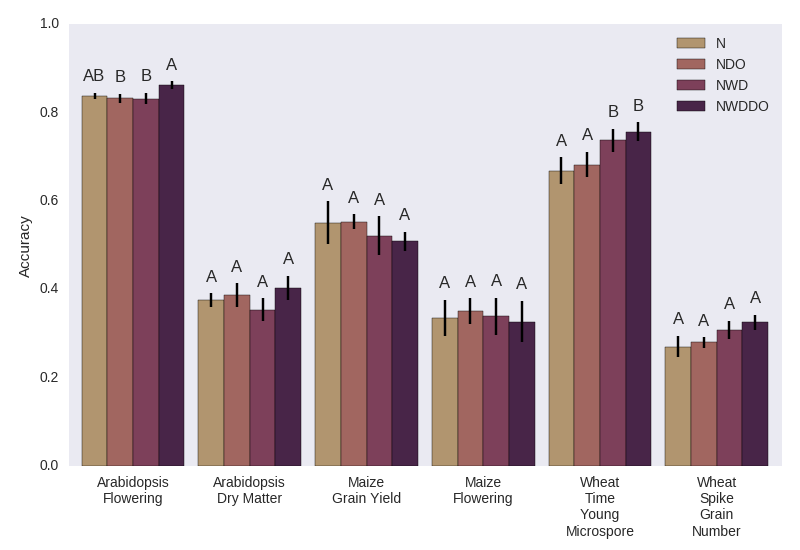
\includegraphics[width=\linewidth]{g3_article/figures/network_comparison.png}
    \caption{Predictive accuracy ($\mu \pm \sigma_{\bar{x}}$) of 
             regularized and non-regularized 
             neural network models for on benchmark datasets. Only the best performing
             network archetecture for each species, trait, and model is included. 
             The accuracy of the best performing model across all folds of data 
             and training cycles were recorded and compared. All pairwise model 
             comparisons within a species and trait were made using a two-sided paired t-test 
             (n=10, paired by training cycle and fold number).
             The resulting p-values were corrected for multiple comparisons within each 
             species and trait combination using the Holm-Bonferroni method. Columns annotated 
             with the same letter are not significantly different 
             at the $\alpha=0.05$ level.}
\label{fig:network-comparison}
\end{figure}
 % Label = fig:network-comparison
\fi

\subsection*{Deep Network Performance}

Contrary to expectation, neural networks with additional hidden layers did not perform
significantly better than networks with a single layer (Figure \ref{fig:depth-comparison}). 
One possible explanation for this observation is that by the universal approximation theorem,
sufficiently large single layer neural networks can approximate any function, including those
that deeper networks can approximate. In this study, single layer networks up to and including
those with 2187 ($3^7$) neurons were evaluated on all datasets. This number is larger than the number
of markers in any dataset evaluated and may be enough to encode complex interactions in only a single
layer.

Networks with deep architectures have proven effective on a wide variety of problems, but the largest
improvements have occurred on problems with high dimensional input data. These include voice recognition 
tasks where vocal frequencies change over a time dimension or two-dimensional images change over 
a time dimension such as in video playback. It is possible that the dimensionality of genomic 
prediction tasks tested are insufficient to benefit from the deep interaction 
effects that have proven effective in prediction tasks in other domains. 

Yet another possibility is that phenotypic measurement error on many datasets is large enough 
to mask the subtle interaction effects that would otherwise be learned by the network.

\ifdefined\showtablesandfigures

\begin{figure}[htbp]
\renewcommand{\familydefault}{\sfdefault}\normalfont
\centering 
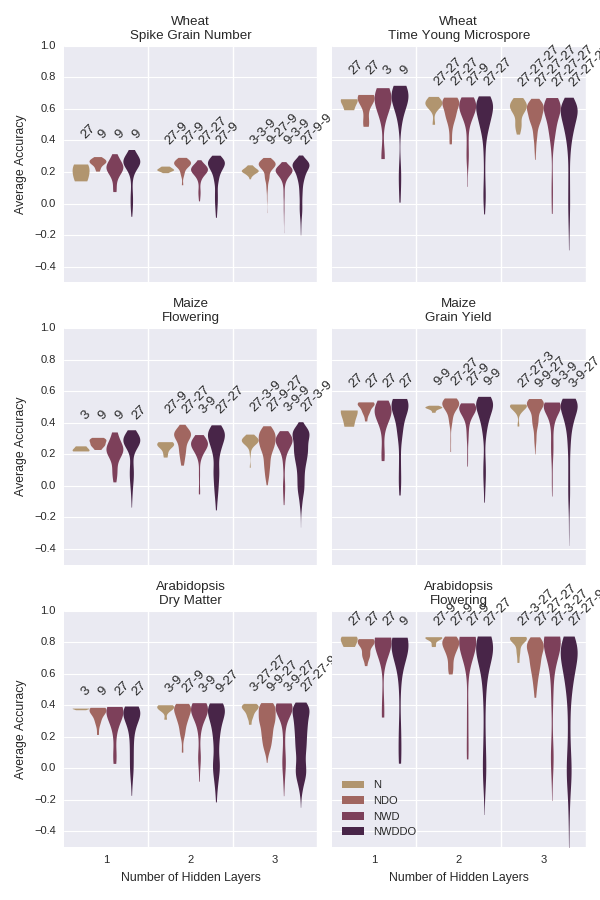
\includegraphics[keepaspectratio,height=\textheight,width=\linewidth]{g3_article/figures/depth_comparison.png}
    \caption{Distribution of predictive accuracy by benchmark dataset, network depth, 
             and model. The violin plot width indicates the Kernel Density Estimate 
             (KDE) of all observed accuracies of all models at a given network depth. 
             The sample size of the KDE is 7, 28, 28, and 112 samples for the 
             N, NWD, NDO, and NWDDO models, respectively. The models contributing 
             to each KDE vary across one or more of five weight decay, five dropout, 
             and seven hidden layer architecture parameters and can be 
             understood as the distribution of results across the set of 
             hyper-parameters to all network models with the same depth and regularization
             type. The KDE bandwidth parameters are set using Scott's normal reference rule. 
             The KDE plots are truncated to the minimum and maximum observed prediction accuracies.} 
\label{fig:depth-comparison}
\end{figure}

 % Label = fig:depth-comparison
\fi

\subsection*{GPU and CPU Training Time}

Network GPU training time was significantly different from CPU training time in all but
one genomic prediction task (Figure \ref{fig:time-comparison}). For small networks 
trained on smaller datasets such as arabidopsis, CPU training completed significantly 
faster than GPU training, though only by a small magnitude. For small networks and 
all other datasets, as well as for all large networks, GPU training time was faster 
than CPU training time on a per-core basis. These results confirm that the previously
observed speedups associated with GPU network training apply to genomic selection applications.

The time required to train a network for genomic prediction is related to
the sample size, marker count, and complexity of the network architecture to be trained.
The improvement in training time when using GPUs for model training was sub-linear across 
all three of these measures. This is because the compute capacity of modern GPUs is 
so large that the processing bottleneck is not the matrix algebra required 
to perform backpropagation but rather the speed of moving data to and from 
the memory on the GPU hardware. We frequently observed CPU utilization of 
100\% during GPU training, indicating that the GPU was demanding resources
at a rate higher than the computer system as a whole could provide them.
Consumer grade GPUs such as the NVIDIA Titan X are now available with twice 
as many CUDA cores as the GTX 680 as well a 50\% wider memory bus, making it potentially
faster than the model used for this analysis. 

It is possible to utilize additional CPU cores to linearly decrease the total time 
needed to train a network, however it is uncommon to utilize multiple GPUs for 
training the same network, and this is not supported by most software packages 
due to limitations in how memory is shared between components in systems with 
multiple GPUs. For example, a quad-core processor like the Intel i7-4790K CPU 
can train a single network approximately four times faster than indicated in 
Figure \ref{fig:time-comparison} if the entire CPU is assigned to a single
network training task. In practice, networks are trained using k-fold
cross validation, so the actual time to fit a family of networks and select
an optimal architecture would be several times larger than these values.
The growth in total time to train when using a CPU suggests that with 
networks larger than the 128x64 network in Figure \ref{fig:time-comparison}, 
CPU training time could become prohibitively large even with quad-core processors. 

Thus, choosing a network training method depends on the size of the dataset and network
to be trained. Low complexity networks train rapidly on CPUs, while larger networks
are more efficiently trained using GPUs. Cloud compute infrastructure providers such 
as Amazon Web Services (AWS) are becoming more popular, and make it much easier
to evaluate training options without purchasing expensive computer hardware.
AWS provides both CPU and GPU rich machines which can be rented at low cost 
and are charged by the hour. This makes it feasible to try CPU and GPU training
on sample data and select a training platform that is most time or cost effective based on the 
complexity of the desired network architecture and the quantity of data available
for training. 

\ifdefined\showtablesandfigures

\begin{figure}[htbp]
\renewcommand{\familydefault}{\sfdefault}\normalfont
\centering 
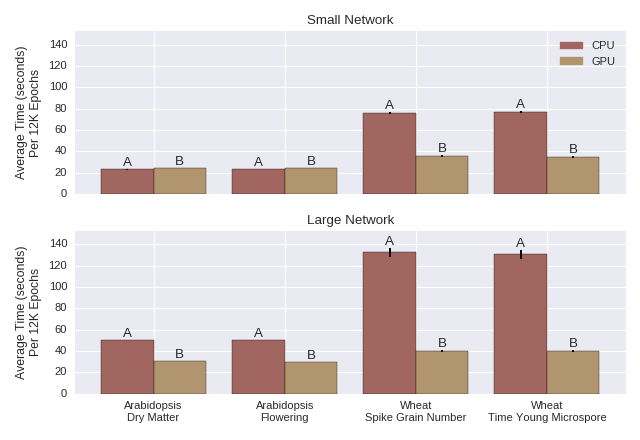
\includegraphics[keepaspectratio,width=\linewidth,height=\textheight]{g3_article/figures/time_comparison.png}
    \caption{Time to train different sized networks on identical datsets using a single dedicated CPU core
             compared to a single dedicated GPU card. Lower time to train is better. For the small network, 
             an unregularized, single hidden layer of 27 neurons was trained for 12K epochs on each dataset. 
             For the large network, two the hidden layers of size 64 and 32 neurons, respectively were trained. 
             Training processes were otherwise equal. This process was repeated ten times per dataset to 
             reduce variation associated with non-deterministic processor scheduling and varying computer system load.
             The ten CPU and GPU training samples were compared using an independent samples T-test with $n=30$. 
             CPU-GPU pairs annotated with the same letter are not significantly different 
             at the $\alpha=0.05$ level.}
\label{fig:time-comparison}
\end{figure}
 % Label = fig:time-comparison
\fi

\subsection*{Overall Conclusion}

Breeders are sometimes interested in predicting the additive genetic value of 
individuals rather than their expressed phenotype. Algorithms such as 
RKHS regression and neural networks often produce genomic prediction 
models with high predictive accuracy because they are able to capture 
interaction effects between genotypes. This is not possible with additive 
linear models such as ridge regression. As a result, caution must be exercised 
when interpreting improved prediction accuracy as a better model in the 
general case. Breeding scenarios where additive genetic value is of primary 
importance may not benefit from the use of models that capture interactions
between genes because these predictions contain non-heritable additive
variation. However, when phenotypic predictions are desirable, such 
as when breeding clonal crop varieties where individual segregates are 
selected to become commercial varieties, models incorporating interaction 
effects should perform better than models capturing only additive effects.

When combined with effective regularization techniques, neural networks can function
as accurate and effective genomic prediction models with a low risk of overfitting
to training data. With the ready availability of GPU computation resources, concerns
over total time to train are partially ameliorated. Searches for optimal architectures or 
regularization techniques can be automated in a time and cost effective 
manner using cloud compute providers such as AWS.



% Chapter #3 - General Conclusions
\chapter{General Conclusions}\label{chp:gen-conclusions}

\section{General Discussion}

There are four primary goals of the work presented in this thesis.

\begin{itemize}
    \item Demonstrate whether neural network models can exhibit competitive 
          accuracy on public datasets.
    \item Explicitly determine the relationship between model regularization and 
          the genetic architecture of traits. 
    \item Determine the effect of adding additional hidden layers to neural 
          network models for genomic prediction.
    \item Explore the effect of GPU computing on neural network training time.
\end{itemize}

To achieve these goals, six public genomic datasets were collected and an
experimental framework was created to test several genomic prediction models.
A combination of CPU and GPU resources were
used to fit nine statistical models including four neural network models
to each of the six datasets while collecting information on training 
time as well as final prediction accuracy. 

Neural networks were top performers on three of the six datasets
presented in this study. While this is a small sample size, it is
sufficient to demonstrate that neural networks can function as 
competitive genomic prediction models. Published studies to date have failed 
to apply regularization to networks, resulting in an underestimation 
of their predictive ability. A large body of work outside of plant 
and animal breeding literature demonstrates that networks can 
rapidly solve complex problems when applied appropriately.
These results provide preliminary evidence that networks can be successful,
but evaluation of regularized networks in comparison with RKHS and 
Bayesian Alphabet methods will be required before drawing conclusions about 
prediction accuracy.

The regularization methods presented in this paper included standard methods such 
as L1 and L2, as well as Bayesian prior distributions and network dropout. 
Given the relationship between regularization, genomic architecture, and model 
performance, it is not surprising that the two unregularized prediction methods, 
ordinary least squares and a standard MLP neural network, were not top performers 
on any dataset (Table \ref{tab:model-comparison}). The performance of the neural 
network models suggests that regularization is critical to achieve optimal 
performance. This is likely to be true for any problem which is predictive rather 
than descriptive in nature.

Adding additional hidden layers to the neural network models did not improve
network performance on the six genomic prediction tasks presented in this study.
This result was unexpected, as similar architectures have resulted in an outstanding 
gain in accuracy on both new and old prediction problems \citep{subasi2005, lang1990, mnih2013}.
There are several possible explanations for these results. First, the universal
approximation theorem predicts that sufficiently large single layer networks
can approximate any function, including those that multi-layer networks can approximate.
However, improved predictive accuracy from deep networks on some categories of problems
in other domains suggests that there are occasions where, 
at a minimum, deep networks train more effectively or reach training states that 
produce better predictive accuracy. It is not clear whether our results imply that
genomic prediction is best performed with neural networks with a single hidden 
layer or whether other neural network types might benefit from additional hidden layers.
A second possibility is that the dimensionality of the genomic prediction problems
presented in the selected datasets was insufficient to take advantage of the
flexible learning process of deep neural networks. Problems where deep networks have
made the largest improvements generally involve data that includes an additional dimension
such as one-dimensional time series or two-dimensional imagery data. Aside from linkage, the markers used as 
input for genomic prediction tasks are mostly independent. It is possible that 
additional data density is required to observe the effects of neural networks, 
such as full sequencing data which has an additional dimensional structure encoded 
in the order of nucleotides along a strand of DNA. A third possibility is that 
the measurement error on the phenotypes examined in this study was sufficiently 
large to mask the subtle interaction effects between markers that a deep 
network could potentially learn. If so, this problem could be resolved by reducing 
measurement error or increasing sampling sizes in genomic prediction training datasets.  

Previous studies have raised concerns about the computational complexity of fitting
neural network models \citep{heslot2012,gonzalez-recio2014}. Our results show
that training neural networks using GPU resources drastically
reduces the rate at which training time grows with sample size, marker count,
and network complexity (Figure \ref{fig:time-comparison}). The improvement in 
training time we observed was so large that growth in total time to train was sub-linear
across all three measures of complexity. This is because the compute capacity 
of modern GPUs is so large that the processing bottleneck is not the matrix calculus
required to fit the model but rather moving data to and from the memory on 
the GPU hardware. Hardware manufacturers are aware of this limitation 
and continue to increase the speed of the hardware 
buses that move data between computer hardware components. Our results
demonstrate that concerns about computation complexity when fitting 
networks are no longer valid on small to medium sized datasets such as 
those presented in this paper. We anticipate that as hardware improves, 
even the largest of datasets will be able to move rapidly between hardware components, 
and the model fitting bottleneck will be capacity of the
GPU to perform algebraic manipulations, much like CPU hardware is for most 
model fitting tasks today.



\section{Future Research}

\subsection*{Other Models}
Future research should directly compare neural network based genomic prediction
models with other state-of-the-art models. The RKHS regression family of models
has performed well on several prediction tasks \citep{heslot2012, crossa2010, gonzalez-recio2014, gianola2006}.
In order to properly evaluate these models, a flexible model fitting
and evaluation model architecture such as the one built for this paper will be
needed. The Bayesian Alphabet models have also performed notably well on
a wide variety of problems \citep{heslot2012, crossa2010, thavamanikumar2015}.
These also should be included in comparisons with regularized neural networks.
Particular focus must be placed on measurable aspects of the genetic architecture 
of a trait that are correlated with the performance of a particular model. This will 
enable better modeling decisions during the development of a genomic selection program.

\subsection*{Other Regularizers}

This study examined the effects of dropout and L2 normalization on neural networks. It 
did not consider alternative regularization techniques which exist for MLP neural
networks. While LASSO regression utilizes L1 regularization and was evaluated, 
L1 regularization on network weights was not evaluated 
to reduce the total number of network parameters evaluated in this study. 
Still other regularizers exist such as activity and bias regularization which 
penalize the total output of all neurons and the bias terms on each neuron, 
respectively. Both of these forms of regularization 
can be applied in an L1 and L2 sense. Another series of regularizers are more commonly
known as constraints, which constrain network various subsets of network parameters 
within bounds, within norms, or to positive real numbers. Unlike many of the 
linear or Bayesian regression techniques evaluated in this and other studies, 
the family of fully-connected neural networks are amenable to dozens of different 
regularization techniques for thousands of different network architectures. This poses
a combinatorics challenge when attempting to select a single optimal network 
architecture. However, this also creates opportunities to identify networks that 
best model the genetic architecture and thus achieve the highest predictive 
accuracy on a given genomic prediction task.

\subsection*{Additional Input Features}

Neural networks are robust to input feature transformations. It is typical 
to transform inputs to a real number in the range $[0,1]$ prior to using 
an input as a model feature. Molecular marker arrays typically output values that
can be linearly scaled within this range, but other values can be easily included
in addition to marker calls. Several methods could be used to encode non-marker information
to improve predictive accuracy. These include location or population information using
a one-hot encoding transformation. Weather information, on daily or weekly intervals could
be included and allowed to interact with marker calls to improve phenotypic estimates.
Sophisticated models such as these could be reverse-engineered to estimate optimal
genetic combinations for performance in particular environments. Like other regression
models, the more features that are included in the model, the more regularization is needed
to prevent overfitting and produce predictive outputs. Many other input features
can be conceived to augment the information leveraged by a network when making
a prediction. While neural networks pose the aforementioned combinatoric architecture
challenge, they are unique in accepting large numbers of inputs from diverse 
sources of data. Practically any information that a human could use when making
a prediction can be transformed to a $[0,1]$ scale and leveraged by a
network. In this way, networks can form so-called expert systems that perform
in ways that are similar to that of a human expert.

\subsection*{Larger Datasets}

This study examined both small and medium density marker datasets. Datasets with
many thousands of marker calls were not included due to time and budgetary constraints.
Future genomic prediction research should include larger datasets with $p \gg n$. Several
examples of these datasets are available in the literature \citep{resende2012, cleveland2012}.

\subsection*{Radial Basis Function Networks}

This work has focused on deep MLP neural networks with sigmoid activation functions.
Architectures such as the Radial Basis Function (RBF) network do not possess the multiple hidden
layers of MLP networks. This alternative architecture is not well studied in the machine learning 
literature, but has shown promising performance on genomic selection 
problems \citep{gonzalez-camacho2012}.

\subsection*{Final Remarks}

Additional research is needed to determine the performance of 
neural networks relative to other state-of-the-art models. This process can
be accelerated by leveraging GPU computation to more quickly evaluate
large numbers of complex networks. As transistor density continues to
increase \citep{moore1965}, and GPU computational capacity subsequently
increases, a network's computational demands will decrease thus making them more
attractive for use in genomic prediction tasks as well as in other domains.





\singlespacing
% References
\newpage
\phantomsection
\addcontentsline{toc}{chapter}{Literature Cited}
%\chapter{Literature Cited}

\bibliographystyle{g3_article/genetics}
\renewcommand\bibname{\MakeUppercase{Literature Cited}}
\bibliography{bibliography}
 
\newpage % Force appendix to start on a new page.

% Appendix A - Raw Data
\phantomsection
\addcontentsline{toc}{chapter}{Appendix A. Raw Data}
\chapter*{Raw Data}

Raw data used in this study was collected from the following publications.

\begin{itemize}
\item Arabidopsis -  \citet{loudet2002}
\item Maize - \citet{crossa2010}
\item Wheat - \citet{thavamanikumar2015}
\end{itemize}

The raw data was collected and processed into a consistent format using a series 
of scripts created to automate data extraction for the analysis presented in
this thesis. The raw data, scripts, and their output as used in all analysis 
in this thesis is available at 
\url{https://github.com/rileymcdowell/genomic-neuralnet/tree/master/genomic\_neuralnet/data}.



% Appendix B - Analysis Code
\phantomsection
\addcontentsline{toc}{chapter}{Appendix B. Analysis Code}
\chapter*{Appendix B. Analysis Code} \label{app:analysis-code}

The source code used to generate the analysis in this paper is available at 
\url{https://github.com/rileymcdowell/genomic-neuralnet}. The \texttt{genomic\_neuralnet}
directory contains the source code itself. The 
\texttt{genomic\_neuralnet/analysis/optimize\_all.sh} script fits all available 
models to all datasets when executed. Command line parameters are available for all python source
code when executed with the \texttt{--help} command line argument. All genomic prediction models presented in this 
paper are implemented in the \texttt{genomic\_neuralnet/methods/} directory. 

To facilitate fitting thousands of model variants on each dataset, Amazon Web Services (AWS) 
resources were utilized for pay by the hour compute capacity. A small compute cluster was 
created containing a single head cluster node and a variable number of slave nodes depending
on the current market price of AWS Elastic Compute Cluster (EC2) instance spot instances at that time.
The head cluster node was initialized with the \texttt{cloud-init-master.sh} script in 
the root source code directory. The slave nodes were initialized
using either the \texttt{cloud-init-slave.sh} or \texttt{cloud-init-slave-gpu.sh} scripts
depending on the absence or presence of a GPU on the node, respectively. All
nodes were running Amazon Linux AMI 2016.03.3 as the base operating system.



% Appendix C - Thesis Code 
\phantomsection
\addcontentsline{toc}{chapter}{Appendix C. Thesis Code}
\chapter*{Thesis Code}

This thesis was generated using the \latex document preparation language. 
All source code files used to generate this paper are available at 
\url{https://github.com/rileymcdowell/genomic-neuralnet-paper}. Generating
this thesis requires a complete working \texttt{texlive} installation.
The \texttt{genomic-neuralnet} library described in
\hyperref[app:analysis-code]{Appendix B}. must also be available on the system for the
figures and tables to be correctly copied into this thesis.





\end{document}
